\documentclass[../main.tex]{subfiles}

\begin{document}

\section{Periféricos y buses externos}

    Los procesadores tienen, por regla general, un gran número de pines disponibles para su conexión con dispositivos externos (de hecho, cuentan con varios miles en los modelos más avanzados). Sin embargo, esta disponibilidad tiene sus limitaciones: en primer lugar, no todos los pines son capaces de realizar todas las funciones. En segundo lugar, el uso de pines concretos requiere un grado de planificación del sistema completo a nivel de placa base. 
        
    Mucha veces querremos la posibilidad de conectar diferentes dispositivos a nuestro diseño, pero no necesariamente que éstos existan desde el comienzo. Por ejemplo, un microcontrolador sencillo puede utilizarse para controlar diferentes tipos de sensores, actuadores, pantallas, controles y, a nivel de diseño, sólo podremos ofrecer unos pocos pines al usuario.

    Para tener la posibilidad de conectar multitud de dispositivos a nuestro procesador, existe el concepto de bus: protocolos que utilizan un conjunto reducido de pines, y permiten, a través de unas pocas líneas de datos, la interconexión de varios (en ocasiones hasta cientos) dispositivos. Dos de los protocolos más extendidos para este propósito son el \textbf{I2C} y \textbf{SPI}.

    \subsection{I2C}

        El \textbf{Bus I2C} (\emph{Inter-Integrated Circuit} es una de estas alternativas. Es de las más sencillas, y permite, a través de únicamente dos líneas, la conexión de hasta 1000 dispositivos. Los elementos más destacables del bus I2C pueden verse en la \Cref{fig:i2c_bus} y son:

        \begin{figure}[hb]
            \centering
            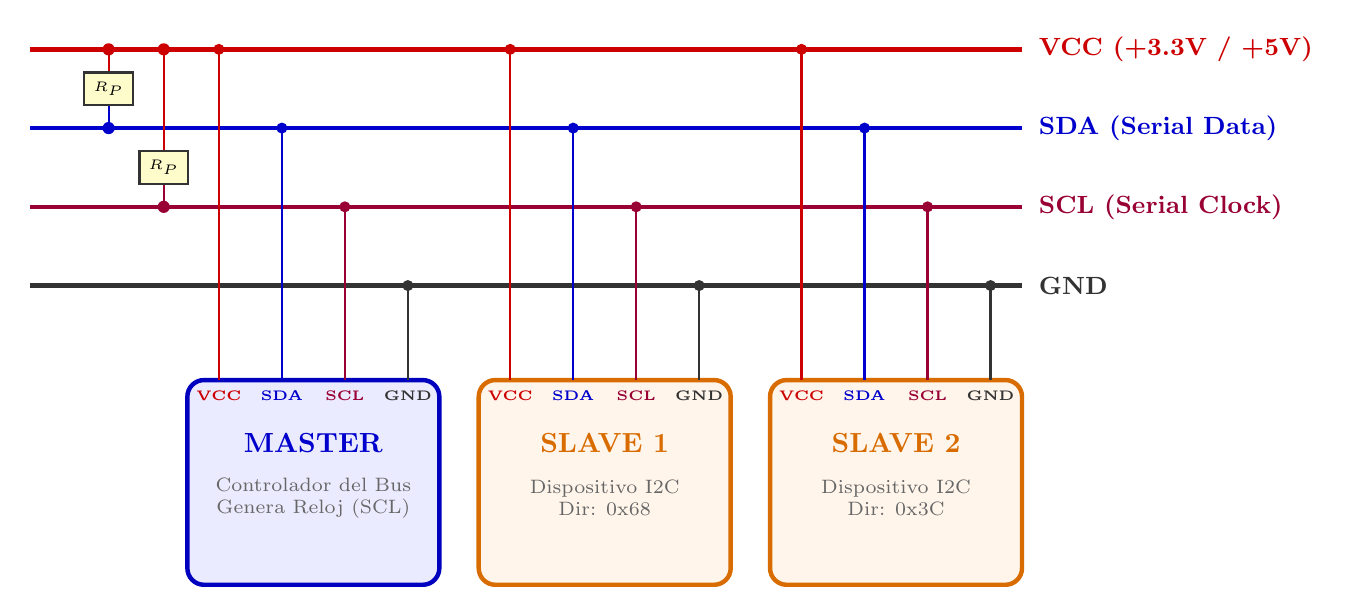
\begin{tikzpicture}[
                font=\sffamily\small,
                % Estilos de los bloques
                master box/.style={
                    draw=blue!75!black,
                    fill=blue!8,
                    ultra thick,
                    rounded corners=6pt,
                    minimum width=3.2cm,
                    minimum height=2.6cm
                },
                slave box/.style={
                    draw=orange!85!black,
                    fill=orange!8,
                    ultra thick,
                    rounded corners=6pt,
                    minimum width=3.2cm,
                    minimum height=2.6cm
                },
                resistor/.style={
                    draw=black!80,
                    fill=yellow!20,
                    thick,
                    minimum width=0.35cm,
                    minimum height=0.35cm,
                    font=\tiny\bfseries
                },
                pin label/.style={
                    font=\tiny\bfseries,
                    inner sep=1pt
                }
            ]

                % --- COORDENADAS Y DE LAS LÍNEAS DEL BUS ---
                \def\yVCC{4.2}
                \def\ySDA{3.2}
                \def\ySCL{2.2}
                \def\yGND{1.2}

                \def\xStart{-0.8}
                \def\xEnd{11.8}

                % --- LÍNEAS PRINCIPALES DEL BUS ---
                \draw[red!80!black, ultra thick] (\xStart, \yVCC) -- (\xEnd, \yVCC) node[right=2pt, font=\bfseries\small] {VCC (+3.3V / +5V)};
                \draw[blue!80!black, ultra thick] (\xStart, \ySDA) -- (\xEnd, \ySDA) node[right=2pt, font=\bfseries\small] {SDA (Serial Data)};
                \draw[purple!80!black, ultra thick] (\xStart, \ySCL) -- (\xEnd, \ySCL) node[right=2pt, font=\bfseries\small] {SCL (Serial Clock)};
                \draw[black!80, ultra thick] (\xStart, \yGND) -- (\xEnd, \yGND) node[right=2pt, font=\bfseries\small] {GND};

                % --- RESISTENCIAS DE PULL-UP (I2C Open-Drain) ---
                \def\xRone{0.2}
                \def\xRtwo{0.9}

                % Pull-up para SDA
                \node[resistor] (R1) at (\xRone, \ySDA + 0.5) {$R_P$};
                \draw[red!80!black, thick] (\xRone, \yVCC) -- (R1.north);
                \draw[blue!80!black, thick] (R1.south) -- (\xRone, \ySDA);
                \fill[red!80!black] (\xRone, \yVCC) circle (2.2pt);
                \fill[blue!80!black] (\xRone, \ySDA) circle (2.2pt);

                % Pull-up para SCL
                \node[resistor] (R2) at (\xRtwo, \ySCL + 0.5) {$R_P$};
                \draw[red!80!black, thick] (\xRtwo, \yVCC) -- (R2.north);
                \draw[purple!80!black, thick] (R2.south) -- (\xRtwo, \ySCL);
                \fill[red!80!black] (\xRtwo, \yVCC) circle (2.2pt);
                \fill[purple!80!black] (\xRtwo, \ySCL) circle (2.2pt);

                % --- DISPOSITIVOS (MASTER Y SLAVES) ---
                % Master
                \def\xM{2.8}
                \node[master box] (master) at (\xM, -1.3) {};
                \node[font=\bfseries, color=blue!80!black] at (\xM, -0.8) {MASTER};
                \node[align=center, font=\scriptsize, color=gray!80!black] at (\xM, -1.5) {Controlador del Bus\\Genera Reloj (SCL)};

                % Slave 1
                \def\xSone{6.5}
                \node[slave box] (slave1) at (\xSone, -1.3) {};
                \node[font=\bfseries, color=orange!85!black] at (\xSone, -0.8) {SLAVE 1};
                \node[align=center, font=\scriptsize, color=gray!80!black] at (\xSone, -1.5) {Dispositivo I2C\\Dir: 0x68};

                % Slave 2
                \def\xStwo{10.2}
                \node[slave box] (slave2) at (\xStwo, -1.3) {};
                \node[font=\bfseries, color=orange!85!black] at (\xStwo, -0.8) {SLAVE 2};
                \node[align=center, font=\scriptsize, color=gray!80!black] at (\xStwo, -1.5) {Dispositivo I2C\\Dir: 0x3C};

                % --- CONEXIONES DE PIN PREDETERMINADAS ---
                \foreach \xDev in {\xM, \xSone, \xStwo} {
                    \def\xVccPin{\xDev - 1.2}
                    \def\xSdaPin{\xDev - 0.4}
                    \def\xSclPin{\xDev + 0.4}
                    \def\xGndPin{\xDev + 1.2}
                    \def\yTop{0.0}

                    % Conexiones verticales a los buses
                    \draw[red!80!black, thick] (\xVccPin, \yTop) -- (\xVccPin, \yVCC);
                    \draw[blue!80!black, thick] (\xSdaPin, \yTop) -- (\xSdaPin, \ySDA);
                    \draw[purple!80!black, thick] (\xSclPin, \yTop) -- (\xSclPin, \ySCL);
                    \draw[black!80, thick] (\xGndPin, \yTop) -- (\xGndPin, \yGND);

                    % Puntos de unión en el bus
                    \fill[red!80!black] (\xVccPin, \yVCC) circle (2pt);
                    \fill[blue!80!black] (\xSdaPin, \ySDA) circle (2pt);
                    \fill[purple!80!black] (\xSclPin, \ySCL) circle (2pt);
                    \fill[black!80] (\xGndPin, \yGND) circle (2pt);

                    % Etiquetas de los pines dentro de las cajas
                    \node[pin label, red!80!black] at (\xVccPin, -0.2) {VCC};
                    \node[pin label, blue!80!black] at (\xSdaPin, -0.2) {SDA};
                    \node[pin label, purple!80!black] at (\xSclPin, -0.2) {SCL};
                    \node[pin label, black!80] at (\xGndPin, -0.2) {GND};
                }

            \end{tikzpicture}
            \caption{Diagrama de un bus I2C}
            \label{fig:i2c_bus}
        \end{figure}

        \begin{itemize}
            \item \emph{Master}: Un único dispositivo que tiene el control del bus, y genera las peticiones en el mismo. El \emph{Master} puede cambiar con ciertas señalizaciones especiales, pero siempre debe ser un único dispositivo.
            \item \emph{Slave}: Pueden ser múltiples, son dispositivos que están conectados al bus y escuchan el mismo a la espera de peticiones del \emph{Master}.
            \item \textbf{SDA} o \emph{Serial Data}: Línea de datos serie, a través de la cual se envía la información (bien del \emph{Master} al \emph{Slave} o viceversa).
            \item \textbf{SCL} o \emph{Serial Clock}: Línea de reloj serie. Controlada por el \emph{Master}, lleva la señal de reloj con la que se sincronizan los datos de \textbf{SDA}. Generalmente, los dispositivos \textbf{I2C} permiten un amplio rango de frecuencias para su funcionamiento, aunque las más típicas son 100 o 400 KHz.
        \end{itemize}

        Un dato interesante a observar es el hecho de que tanto \textbf{SCL} como \textbf{SDA} tienen resistencia de \emph{pull-up} a VCC. Es decir, que por defecto están siempre a ``1''. Cualquier dispositivo que se conecte, operará en modo de \emph{colector abierto} (open drain). Es decir, que únicamente podrá bajar la línea a ``0'' conectándola a tierra, enviándose los ``unos'' pasivamente.

        \subsubsection{Funcionamiento del bus I2C - capa física}

            Una vez realizadas las conexiones entre los dispositivos, la siguiente pregunta razonable es cómo opera el bus I2C. Las transferencias de datos siguen, de manera general, los siguientes pasos:

            \begin{enumerate}
                \item Una transferencia se inicia con una condición de inicio (\textbf{S} (start)), que se señala desde el \emph{Master} bajando \textbf{SDA} a ``0'', mientras \textbf{SCL} se mantiene a ``1''.
                \item A continuación \textbf{SCL} comienza a oscilar, bajando a ``0'' en primer lugar, mientras se prepara el bit a enviar en \textbf{SDA}.
                \item Cuando \textbf{SCL} sube a 1, el bit enviado está disponible en \textbf{SDA} y el resto de dispositivos \emph{Slaves} pueden leerlo. 
                \item Se repiten los pasos 2 y 3 tantas veces sea necesario para enviar todos los bits.
                \item El último bit es seguido de un pulso de reloj sin dato, en el cual \textbf{SDA} se pone a ``0''.
                \item Finalmente, se indica la condición de fin (\textbf{P} (stop)), liberando primero \textbf{SCL}, y posteriormente \textbf{SDA}.
            \end{enumerate}

            Este proceso se puede ver gráficamente en la \Cref{fig:i2c_transfer}.
            
            \begin{figure}[h]
                \centering
                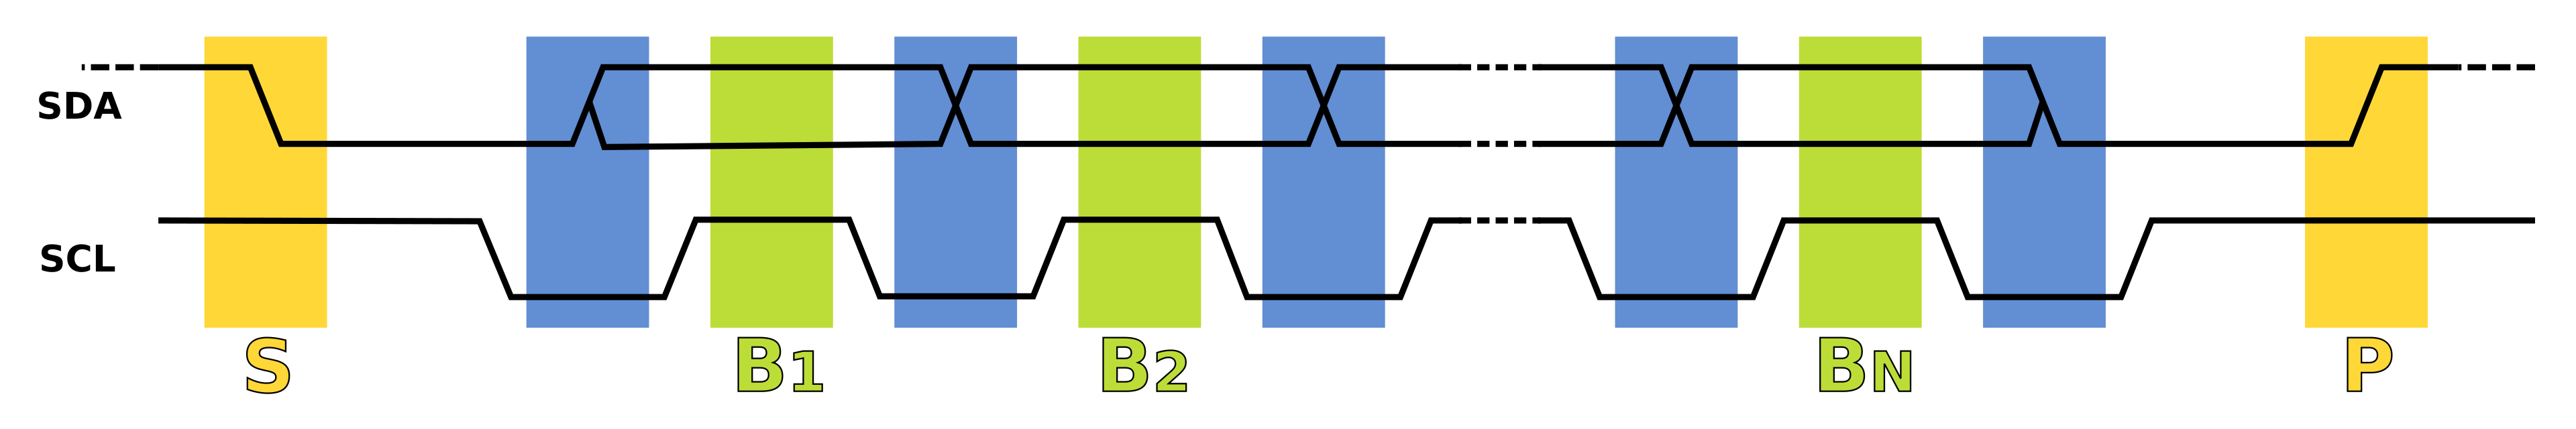
\includegraphics[width=\textwidth]{res/I2C_data_transfer.png}
                \caption{Transferencia de datos en I2C. (fuente:wikipedia)}
                \label{fig:i2c_transfer}
            \end{figure}

        \subsubsection{Direccionamiento en I2C - capa lógica}\label{subsub:i2clogic}
            
            Ahora bien, dentro de estas transferencias, ¿cómo sabemos a qué dispositivo van los bits? para ello, cada \emph{Slave} cuenta con una dirección (de 7 bits, o 10 en versiones más modernas), habitualmente fijada por hardware, y con la que se puede identificar un dispositivo concreto. Así, para escribir, se seguirá el siguiente procedimiento:

            \begin{enumerate}
                \item Inicio de comunicación con condición inicial \textbf{S} seguida de la dirección (7 bits) + bit ``0'' (write). \emph{Slave} responde \textbf{ACK}.
                \item Envío del comando (o registro destino) (8 bits). \emph{Slave} responde \textbf{ACK}.
                \item Envío del dato (8 bits). \emph{Slave} responde \textbf{ACK}.
                \item Generalmente, y según dispositivo, se pueden enviar datos consecutivos que irán a parar a registros consecutivos si se quiere.
                \item Fin de comunicación con condición de parada \textbf{P}.
            \end{enumerate}

            Para leer, el proceso es algo más complejo, ya que primero indicaremos el registro en modo escritura, y posteriormente cederemos el control al \emph{Slave} en modo lectura para que nos pase el dato por el bus.

            \begin{enumerate}
                \item Inicio de comunicación con condición inicial \textbf{S} seguida de la dirección (7 bits) + bit ``0'' (write). \emph{Slave} responde \textbf{ACK}.
                \item Envío del comando (o registro destino) (8 bits). \emph{Slave} responde \textbf{ACK}.
                \item Re-Inicio de comunicación con condición inicial \textbf{S} seguida de la dirección (7 bits) + bit ``1'' (read). \emph{Slave} responde \textbf{ACK}.
                \item El \emph{Slave} toma el control y envía el dato de vuelta (8 bits). El \emph{Master} puede responder con \textbf{ACK} para pedir más datos consecutivos, o con \textbf{NACK} para terminar la comunicación.
                \item Fin de comunicación con condición de parada \textbf{P}.
            \end{enumerate}

            Las condiciones \textbf{ACK} y \textbf{NACK} se indican, respectivamente, con un ``0'' y un ``1'' (sí, están invertidas) por parte del receptor, en la línea \textbf{SDA} tras las transmisión de un byte.

            El proceso para ambas transacciones puede observarse en la \Cref{fig:i2c_read_write}

            \definecolor{masterBG}{HTML}{EBF5FB}
            \definecolor{masterBORDER}{HTML}{2980B9}
            \definecolor{slaveBG}{HTML}{FEF9E7}
            \definecolor{slaveBORDER}{HTML}{D68910}
            \definecolor{ctrlBG}{HTML}{FDEDEC}
            \definecolor{ctrlBORDER}{HTML}{CB4335}

            \tikzset{
                i2cbase/.style={
                    draw, 
                    minimum height=0.9cm, 
                    font=\sffamily\scriptsize, 
                    align=center, 
                    outer sep=0pt, 
                    line width=0.6pt
                },
                master/.style={i2cbase, fill=masterBG, draw=masterBORDER, text=masterBORDER!40!black},
                slave/.style={i2cbase, fill=slaveBG, draw=slaveBORDER, text=slaveBORDER!40!black},
                ctrl/.style={i2cbase, fill=ctrlBG, draw=ctrlBORDER, text=ctrlBORDER!40!black, font=\sffamily\bfseries\scriptsize},
                opt/.style={i2cbase, fill=masterBG!30, draw=masterBORDER, dashed, text=masterBORDER!40!black},
                title/.style={font=\sffamily\bfseries\small, text=gray!90!black},
                stepnum/.style={font=\sffamily\bfseries\tiny, text=gray!70!black},
                legendtext/.style={font=\sffamily\tiny, text=gray!80!black}
            }

            \begin{figure}[h!]
                \centering
                \begin{tikzpicture}
                    \node[ctrl, minimum height=0.4cm, minimum width=0.6cm] (l1) {};
                    \node[legendtext, right=3pt of l1] {Inicio / Fin (Master)};
                    
                    \node[master, minimum height=0.4cm, minimum width=0.6cm, right=100pt of l1] (l2) {};
                    \node[legendtext, right=3pt of l2] {Generado por \textbf{Master}};
                    
                    \node[slave, minimum height=0.4cm, minimum width=0.6cm, right=100pt of l2] (l3) {};
                    \node[legendtext, right=3pt of l3] {Generado por \textbf{Slave}};
                \end{tikzpicture}
                \resizebox{\linewidth}{!}{%
                \begin{tikzpicture}[node distance=0pt]

                    % Título del diagrama
                    \node[title, anchor=west] (t1) at (0, 1.3) {1. Escritura en I2C (Write)};

                    % Bloques del protocolo de escritura
                    \node[ctrl, minimum width=0.6cm] (w_s) at (0,0) {\textbf{S}};
                    \node[master, right=-0.6pt of w_s, minimum width=1.8cm] (w_addr) {Dirección Slave\\(7 bits)};
                    \node[master, right=-0.6pt of w_addr, minimum width=0.7cm] (w_bit) {0\\(W)};
                    \node[slave, right=-0.6pt of w_bit, minimum width=0.9cm] (w_ack1) {\textbf{ACK}\\(0)};
                    \node[master, right=-0.6pt of w_ack1, minimum width=2.2cm] (w_reg) {Registro / Cmd\\(8 bits)};
                    \node[slave, right=-0.6pt of w_reg, minimum width=0.9cm] (w_ack2) {\textbf{ACK}\\(0)};
                    \node[master, right=-0.6pt of w_ack2, minimum width=1.8cm] (w_data) {Dato\\(8 bits)};
                    \node[slave, right=-0.6pt of w_data, minimum width=0.9cm] (w_ack3) {\textbf{ACK}\\(0)};
                    \node[opt, right=-0.6pt of w_ack3, minimum width=1.8cm] (w_dataN) {Dato N (opc.)\\(8 bits)};
                    \node[slave, right=-0.6pt of w_dataN, minimum width=0.9cm] (w_ackN) {\textbf{ACK}\\(0)};
                    \node[ctrl, right=-0.6pt of w_ackN, minimum width=0.6cm] (w_p) {\textbf{P}};

                    % Indicadores de pasos
                    \node[stepnum, above=3pt of w_s] {Paso 1};
                    \node[stepnum, above=3pt of w_addr] {Paso 2};
                    \node[stepnum, above=3pt of w_reg] {Paso 3};
                    \node[stepnum, above=3pt of w_data] {Paso 4};
                    \node[stepnum, above=3pt of w_dataN] {Paso 5};
                    \node[stepnum, above=3pt of w_p] {Paso 6};

                \end{tikzpicture}%
                }
                \vspace{0.8cm}
                \resizebox{\linewidth}{!}{%
                \begin{tikzpicture}[node distance=0pt]

                    % Título del diagrama
                    \node[title, anchor=west] (t2) at (0, 1.3) {2. Lectura en I2C (Read)};

                    % Bloques del protocolo de lectura
                    \node[ctrl, minimum width=0.6cm] (r_s) at (0,0) {\textbf{S}};
                    \node[master, right=-0.6pt of r_s, minimum width=1.7cm] (r_addr1) {Dirección Slave\\(7 bits)};
                    \node[master, right=-0.6pt of r_addr1, minimum width=0.6cm] (r_w) {0\\(W)};
                    \node[slave, right=-0.6pt of r_w, minimum width=0.8cm] (r_ack1) {\textbf{ACK}\\(0)};
                    \node[master, right=-0.6pt of r_ack1, minimum width=2.0cm] (r_reg) {Registro / Cmd\\(8 bits)};
                    \node[slave, right=-0.6pt of r_reg, minimum width=0.8cm] (r_ack2) {\textbf{ACK}\\(0)};
                    \node[ctrl, right=-0.6pt of r_ack2, minimum width=0.6cm] (r_sr) {\textbf{Sr}};
                    \node[master, right=-0.6pt of r_sr, minimum width=1.7cm] (r_addr2) {Dirección Slave\\(7 bits)};
                    \node[master, right=-0.6pt of r_addr2, minimum width=0.6cm] (r_r) {1\\(R)};
                    \node[slave, right=-0.6pt of r_r, minimum width=0.8cm] (r_ack3) {\textbf{ACK}\\(0)};
                    \node[slave, right=-0.6pt of r_ack3, minimum width=1.8cm] (r_data) {Dato Slave\\(8 bits)};
                    \node[master, right=-0.6pt of r_data, minimum width=1.0cm] (r_nack) {\textbf{NACK}\\(1)};
                    \node[ctrl, right=-0.6pt of r_nack, minimum width=0.6cm] (r_p) {\textbf{P}};

                    % Indicadores de pasos
                    \node[stepnum, above=3pt of r_s] {Paso 1};
                    \node[stepnum, above=3pt of r_addr1] {Paso 2};
                    \node[stepnum, above=3pt of r_reg] {Paso 3};
                    \node[stepnum, above=3pt of r_sr] {Paso 4};
                    \node[stepnum, above=3pt of r_addr2] {Paso 5};
                    \node[stepnum, above=3pt of r_data] {Paso 6};
                    \node[stepnum, above=3pt of r_p] {Paso 7};

                \end{tikzpicture}%
                }
                \caption{Escrituras y lecturas, respectivamente, en I2C}
                \label{fig:i2c_read_write}
            \end{figure}
                    
        \subsubsection{Líneas auxiliares a I2C}

            En ocasiones, utilizar únicamente las líneas \textbf{SCL} y \textbf{SDA} no es suficiente. Pensemos por ejemplo en el caso de las interrupciones. Con tan sólo las dos líneas de I2C, capturar una interrupción es imposible, tendríamos que hacer una encuesta activa a los periféricos, preguntando periódicamente si tienen algún dato de interés. Esto sería claramente ineficiente.

            Es por ello que las interrupciones de los dispositivos sí van por líneas separadas, para que el procesador sea capaz de capturarlas, identificar directamente el dispositivo causante, y entonces, y sólo entonces, encuestarlo vía I2C para recibir el dato. Adicionalmente, algunos dispositivos disponen de otras señales extra, para por ejemplo habilitarlos o resetearlos.

    \subsection{SPI}

        El \textbf{Bus SPI} (\emph{Serial Peripheral Interface}) es un protocolo de comunicación serie síncrono diseñado para la interconexión de componentes a corta distancia dentro de una misma placa (si bien también se utiliza entre placas cercanas). A diferencia de I2C, SPI es un bus \emph{Full Duplex} (permite transmitir y recibir datos de manera simultánea) y no utiliza un direccionamiento por software, sino líneas físicas dedicadas para seleccionar cada periférico.

        Los elementos principales del bus SPI y sus conexiones típicas se resumen en la \Cref{fig:spi_bus}:

        \definecolor{misoColor}{HTML}{008080}

        \begin{figure}[hb]
            \centering
            \resizebox{\linewidth}{!}{%
            \begin{tikzpicture}[
                font=\sffamily\small,
                master box/.style={
                    draw=blue!75!black,
                    fill=blue!8,
                    ultra thick,
                    rounded corners=6pt,
                    minimum width=4.0cm,
                    minimum height=2.6cm
                },
                slave box/.style={
                    draw=orange!85!black,
                    fill=orange!8,
                    ultra thick,
                    rounded corners=6pt,
                    minimum width=3.4cm,
                    minimum height=2.6cm
                },
                pin label/.style={
                    font=\tiny\bfseries,
                    inner sep=1pt
                }
            ]

                % --- COORDENADAS Y DE LAS LÍNEAS DEL BUS ---
                \def\yVCC{5.0}
                \def\ySCLK{4.2}
                \def\yMOSI{3.4}
                \def\yMISO{2.6}
                \def\yGND{1.8}

                \def\xStart{-0.5}
                \def\xEnd{12.2}

                % --- LÍNEAS PRINCIPALES DEL BUS ---
                \draw[red!80!black, ultra thick] (\xStart, \yVCC) -- (\xEnd, \yVCC) node[right=2pt, font=\bfseries\small] {VCC (+3.3V / +5V)};
                \draw[purple!80!black, ultra thick] (\xStart, \ySCLK) -- (\xEnd, \ySCLK) node[right=2pt, font=\bfseries\small] {SCLK (Serial Clock)};
                \draw[blue!80!black, ultra thick] (\xStart, \yMOSI) -- (\xEnd, \yMOSI) node[right=2pt, font=\bfseries\small] {MOSI (Master Out Slave In)};
                \draw[misoColor, ultra thick] (\xStart, \yMISO) -- (\xEnd, \yMISO) node[right=2pt, font=\bfseries\small] {MISO (Master In Slave Out)};
                \draw[black!80, ultra thick] (\xStart, \yGND) -- (\xEnd, \yGND) node[right=2pt, font=\bfseries\small] {GND};

                % --- DISPOSITIVOS (MASTER Y SLAVES) ---
                % Master
                \def\xM{2.2}
                \node[master box] (master) at (\xM, -0.8) {};
                \node[font=\bfseries, color=blue!80!black] at (\xM, -0.3) {MASTER};
                \node[align=center, font=\scriptsize, color=gray!80!black] at (\xM, -1.1) {Controlador del Bus\\Genera SCLK y CS};

                % Slave 1
                \def\xSone{6.8}
                \node[slave box] (slave1) at (\xSone, -0.8) {};
                \node[font=\bfseries, color=orange!85!black] at (\xSone, -0.3) {SLAVE 1};
                \node[align=center, font=\scriptsize, color=gray!80!black] at (\xSone, -1.1) {Periférico SPI 1\\(p.~ej. Pantalla LCD)};

                % Slave 2
                \def\xStwo{10.6}
                \node[slave box] (slave2) at (\xStwo, -0.8) {};
                \node[font=\bfseries, color=orange!85!black] at (\xStwo, -0.3) {SLAVE 2};
                \node[align=center, font=\scriptsize, color=gray!80!black] at (\xStwo, -1.1) {Periférico SPI 2\\(p.~ej. Memoria Flash)};

                % --- PINES Y CONEXIONES DEL MASTER ---
                \def\yTop{0.5}

                \def\xMvcc{\xM - 1.5}
                \def\xMsclk{\xM - 1.0}
                \def\xMmosi{\xM - 0.5}
                \def\xMmiso{\xM + 0.0}
                \def\xMcsone{\xM + 0.5}
                \def\xMcstwo{\xM + 1.0}
                \def\xMgnd{\xM + 1.5}

                \draw[red!80!black, thick] (\xMvcc, \yTop) -- (\xMvcc, \yVCC);
                \draw[purple!80!black, thick] (\xMsclk, \yTop) -- (\xMsclk, \ySCLK);
                \draw[blue!80!black, thick] (\xMmosi, \yTop) -- (\xMmosi, \yMOSI);
                \draw[misoColor, thick] (\xMmiso, \yTop) -- (\xMmiso, \yMISO);
                \draw[black!80, thick] (\xMgnd, \yTop) -- (\xMgnd, \yGND);

                \fill[red!80!black] (\xMvcc, \yVCC) circle (2pt);
                \fill[purple!80!black] (\xMsclk, \ySCLK) circle (2pt);
                \fill[blue!80!black] (\xMmosi, \yMOSI) circle (2pt);
                \fill[misoColor] (\xMmiso, \yMISO) circle (2pt);
                \fill[black!80] (\xMgnd, \yGND) circle (2pt);

                %\node[pin label, red!80!black] at (\xMvcc, 0.3) {VCC};
                %\node[pin label, purple!80!black] at (\xMsclk, 0.3) {SCLK};
                %\node[pin label, blue!80!black] at (\xMmosi, 0.3) {MOSI};
                %\node[pin label, misoColor] at (\xMmiso, 0.3) {MISO};
                \node[pin label, orange!80!black] at (\xMcsone, 0.3) {CS1};
                \node[pin label, magenta!80!black] at (\xMcstwo, 0.3) {CS2};
                %\node[pin label, black!80] at (\xMgnd, 0.3) {GND};

                % --- SLAVE 1 PINES & CONEXIONES ---
                \def\xSonevcc{\xSone - 1.25}
                \def\xSonesclk{\xSone - 0.75}
                \def\xSonemosi{\xSone - 0.25}
                \def\xSonemiso{\xSone + 0.25}
                \def\xSonecs{\xSone + 0.75}
                \def\xSonegnd{\xSone + 1.25}

                \draw[red!80!black, thick] (\xSonevcc, \yTop) -- (\xSonevcc, \yVCC);
                \draw[purple!80!black, thick] (\xSonesclk, \yTop) -- (\xSonesclk, \ySCLK);
                \draw[blue!80!black, thick] (\xSonemosi, \yTop) -- (\xSonemosi, \yMOSI);
                \draw[misoColor, thick] (\xSonemiso, \yTop) -- (\xSonemiso, \yMISO);
                \draw[black!80, thick] (\xSonegnd, \yTop) -- (\xSonegnd, \yGND);

                \fill[red!80!black] (\xSonevcc, \yVCC) circle (2pt);
                \fill[purple!80!black] (\xSonesclk, \ySCLK) circle (2pt);
                \fill[blue!80!black] (\xSonemosi, \yMOSI) circle (2pt);
                \fill[misoColor] (\xSonemiso, \yMISO) circle (2pt);
                \fill[black!80] (\xSonegnd, \yGND) circle (2pt);

                %\node[pin label, red!80!black] at (\xSonevcc, 0.3) {VCC};
                %\node[pin label, purple!80!black] at (\xSonesclk, 0.3) {SCLK};
                %\node[pin label, blue!80!black] at (\xSonemosi, 0.3) {MOSI};
                %\node[pin label, misoColor] at (\xSonemiso, 0.3) {MISO};
                \node[pin label, orange!80!black] at (\xSonecs, 0.3) {CS};
                %\node[pin label, black!80] at (\xSonegnd, 0.3) {GND};

                % --- SLAVE 2 PINES & CONEXIONES ---
                \def\xStwovcc{\xStwo - 1.25}
                \def\xStwosclk{\xStwo - 0.75}
                \def\xStwomosi{\xStwo - 0.25}
                \def\xStwomiso{\xStwo + 0.25}
                \def\xStwocs{\xStwo + 0.75}
                \def\xStwognd{\xStwo + 1.25}

                \draw[red!80!black, thick] (\xStwovcc, \yTop) -- (\xStwovcc, \yVCC);
                \draw[purple!80!black, thick] (\xStwosclk, \yTop) -- (\xStwosclk, \ySCLK);
                \draw[blue!80!black, thick] (\xStwomosi, \yTop) -- (\xStwomosi, \yMOSI);
                \draw[misoColor, thick] (\xStwomiso, \yTop) -- (\xStwomiso, \yMISO);
                \draw[black!80, thick] (\xStwognd, \yTop) -- (\xStwognd, \yGND);

                \fill[red!80!black] (\xStwovcc, \yVCC) circle (2pt);
                \fill[purple!80!black] (\xStwosclk, \ySCLK) circle (2pt);
                \fill[blue!80!black] (\xStwomosi, \yMOSI) circle (2pt);
                \fill[misoColor] (\xStwomiso, \yMISO) circle (2pt);
                \fill[black!80] (\xStwognd, \yGND) circle (2pt);

                %\node[pin label, red!80!black] at (\xStwovcc, 0.3) {VCC};
                %\node[pin label, purple!80!black] at (\xStwosclk, 0.3) {SCLK};
                %\node[pin label, blue!80!black] at (\xStwomosi, 0.3) {MOSI};
                %\node[pin label, misoColor] at (\xStwomiso, 0.3) {MISO};
                \node[pin label, magenta!80!black] at (\xStwocs, 0.3) {CS};
                %\node[pin label, black!80] at (\xStwognd, 0.3) {GND};

                % --- LÍNEAS DEDICADAS DE CHIP SELECT (CS1 y CS2) ---
                \draw[orange!80!black, thick] (\xMcsone, \yTop) -- (\xMcsone, 1.1) -- (\xSonecs, 1.1) -- (\xSonecs, \yTop);
                \fill[orange!80!black] (\xMcsone, \yTop) circle (1.5pt);
                \fill[orange!80!black] (\xSonecs, \yTop) circle (1.5pt);

                \draw[magenta!80!black, thick] (\xMcstwo, \yTop) -- (\xMcstwo, 0.7) -- (\xStwocs, 0.7) -- (\xStwocs, \yTop);
                \fill[magenta!80!black] (\xMcstwo, \yTop) circle (1.5pt);
                \fill[magenta!80!black] (\xStwocs, \yTop) circle (1.5pt);

            \end{tikzpicture}%
            }
            \caption{Diagrama de un bus SPI en configuración de selección independiente}
            \label{fig:spi_bus}
        \end{figure}

        \begin{itemize}
            \item \emph{Master}: Dispositivo controlador que inicia las transacciones, genera la señal de reloj principal (\textbf{SCLK}) y gestiona las líneas de selección de cada esclavo \textbf{CSx}.
            \item \emph{Slave}: Dispositivos receptores/emisores. Únicamente están atentos a la información del bus cuando su señal individual de \textbf{CSx} está activa. Así se asegura exclusividad en las líneas del bus siempre y cuando el \emph{Master} lo gestione de manera adecuada.
            \item \textbf{SCLK} (\emph{Serial Clock}): Línea de reloj generada por el \emph{Master}. A diferencia de \textbf{I2C}, \textbf{SPI} no define un límite estricto de velocidad y suele trabajar a frecuencias más altas (en el entorno de MHz).
            \item \textbf{MOSI} (\emph{Master Out Slave In}): Línea serie para el envío de datos desde el \emph{Master} hacia el \emph{Slave}.
            \item \textbf{MISO} (\emph{Master In Slave Out}): Línea serie para la recepción de datos en el \emph{Master} provenientes del \emph{Slave}.
            \item \textbf{CS} (\emph{Chip Select}): Líneas dedicadas e independientes (activas a nivel bajo, ``0'') para habilitar el \emph{Slave} concreto con el que se desea comunicar.
        \end{itemize}

        \subsubsection{Funcionamiento del bus SPI - capa física}

            A diferencia de las líneas con \emph{pull-up} de I2C, SPI utiliza salidas activas controladas por el \emph{Master}. Esto elimina la necesidad de las resistencias, permitiendo velocidades mayores (debido a tiempos de conmutación más rápidos).

            La información que atraviesa las líneas \textbf{MOSI} y \textbf{MISO} se almacena con registros de desplazamiento, en los que la unidad de transferencia básica es un byte completo. 

            Por cada pulso introducido en \textbf{SCLK}:
            \begin{enumerate}
                \item El \emph{Master} desplaza un bit hacia el \emph{Slave} por la línea \textbf{MOSI}.
                \item Simultáneamente, el \emph{Slave} desplaza un bit hacia el \emph{Master} por la línea \textbf{MISO}.
                \item Tras 8 ciclos de reloj, ambos dispositivos han transferido un byte completo.
            \end{enumerate}

            \paragraph{Modos de transmisión SPI (CPOL y CPHA):}
            Los dispositivos definen su modo de operación en función de dos parámetros configurables en el hardware:

            \begin{itemize}
                \item \textbf{CPOL} (\emph{Clock Polarity}): Define el estado de reposo de la línea de reloj \textbf{SCLK}. Si $\text{CPOL}=0$, la línea reposa en ``0'' lógico; si $\text{CPOL}=1$, reposa en ``1''.
                \item \textbf{CPHA} (\emph{Clock Phase}): Define en qué flanco del reloj se capturan los datos. Si $\text{CPHA}=0$, los datos se muestrean en el primer flanco y se muestrean en el segundo; si $\text{CPHA}=1$, al contrario.
            \end{itemize}

            La combinación de ambos parámetros da lugar a los 4 modos SPI estándar:

            \begin{table}[h!]
                \centering
                \small
                \sffamily
                \begin{tabular}{cccccc}
                    \hline
                    \textbf{Modo SPI} & \textbf{CPOL} & \textbf{CPHA} & \textbf{Reloj en reposo} & \textbf{Flanco de Muestreo} \\ \hline
                    \textbf{Modo 0} & 0 & 0 & Nivel Bajo (0) & Flanco de subida \\
                    \textbf{Modo 1} & 0 & 1 & Nivel Bajo (0) & Flanco de bajada \\
                    \textbf{Modo 2} & 1 & 0 & Nivel Alto (1) & Flanco de bajada \\
                    \textbf{Modo 3} & 1 & 1 & Nivel Alto (1) & Flanco de subida \\ \hline
                \end{tabular}
                \caption{Modos de funcionamiento en el protocolo SPI}
                \label{tab:spi_modes}
            \end{table}

        \subsubsection{Funcionamiento del bus SPI - capa lógica}

            Una vez se transmite un byte, su significado no tiene una descripción en el estándar (como sí tiene \textbf{I2C}), y depende del fabricante del dispositivo el definir su comportamiento. Habitualmente, el primer byte enviado contendrá el comando que ejecutar o la dirección a la que escribir, mientras que los bytes siguientes serán los datos a transmitir. No obstante es importante recalcar que el funcionamiento específico dependerá del periférico conectado.

        \subsubsection{Topologías de conexión}

            A nivel de diseño de hardware, existen dos métodos principales para interconectar múltiples periféricos SPI a un mismo controlador:

            \begin{enumerate}
                \item \textbf{(\emph{Independent Slave / Parallel Configuration}):} Es la topología estándar vista en la \Cref{fig:spi_bus}. Las líneas de reloj y datos son compartidas por todos los periféricos, pero el controlador necesita una línea \textbf{CSx} dedicada para cada esclavo.
                \item \textbf{(\emph{Daisy Chain Configuration}):} En dispositivos diseñados específicamente para ello, la salida \textbf{MISO} de un esclavo se conecta a la entrada \textbf{MOSI} del siguiente. De este modo, una única línea \textbf{CS} común activa todos los esclavos a la vez. La información se pasa de uno a otro secuencialmente como un único gran registro de desplazamiento.
            \end{enumerate}


    \subsection{Dispositivos externos mapeados en memoria (FMC)}

        En los buses serie como \textbf{I2C} o \textbf{SPI}, los comandos y datos se envían de forma secuencial, a través de un número reducido de hilos. A nivel de software, esto se traduce en drivers que deben, poco a poco, enviar y recibir toda la información que se desee. Esto es notablemente más complicado que el trabajo con los periféricos integrados del procesador, cuyos registros se mapean directamente en memoria.

        Para dispositivos externos con gran cantidad de registros (o directamente, memorias), los microcontroladores actuales suelen incorporar periféricos dedicados que permiten mapear, en el propio espacio de memoria del procesador, el mapa de memoria del dispositivo externo. Esto facilita enormemente la interacción. Por ejemplo, uno muy habitual es el \PER{FMC} (\emph{Flexible Memory Controller}).

        Lo hacen conectando el bus interno del procesador directamente con un bus paralelo externo (bus de direcciones, bus de datos y líneas de control) mediante un controlador de memoria intermedio que realiza las traducciones de un espacio de direcciones al otro. Así, el acceso al dispositivo se realiza mediante instrucciones estándar de lectura y escritura en C, exactamente como si se tratara de la memoria RAM o Flash internas. Se muestra un esquema en la \Cref{fig:fmc_bus}:

        \begin{figure}[hb]
            \centering
            \resizebox{\linewidth}{!}{%
            \begin{tikzpicture}[
                font=\sffamily\small,
                mcu box/.style={
                    draw=blue!75!black,
                    fill=blue!4,
                    ultra thick,
                    rounded corners=8pt,
                    minimum width=7.2cm,
                    minimum height=3.2cm
                },
                cpu box/.style={
                    draw=blue!80!black,
                    fill=blue!12,
                    thick,
                    rounded corners=5pt,
                    minimum width=2.5cm,
                    minimum height=2.0cm,
                    align=center,
                    font=\sffamily\scriptsize
                },
                fmc box/.style={
                    draw=blue!90!black,
                    fill=blue!22,
                    thick,
                    rounded corners=5pt,
                    minimum width=2.8cm,
                    minimum height=2.0cm,
                    align=center,
                    font=\sffamily\scriptsize
                },
                dev box/.style={
                    draw=orange!85!black,
                    fill=orange!8,
                    ultra thick,
                    rounded corners=8pt,
                    minimum width=4.0cm,
                    minimum height=3.2cm
                },
                pin label/.style={
                    font=\tiny\bfseries,
                    inner sep=1pt
                }
            ]

                % --- COORDENADAS Y DE LAS LÍNEAS DEL BUS PARALELO EXTERNO ---
                \def\yADDR{3.2}
                \def\yDATA{2.6}
                \def\yNE{1.8}

                \def\xStart{-0.5}
                \def\xEnd{12.2}

                % --- LÍNEAS / BUSES PRINCIPALES EXTERNOS ---
                \draw[purple!80!black, line width=2.5pt] (\xStart, \yADDR) -- (\xEnd, \yADDR) node[right=2pt, font=\bfseries\small] {Bus de Direcciones Ext. ($A[0..N]$)};
                \draw[blue!80!black, line width=2.5pt] (\xStart, \yDATA) -- (\xEnd, \yDATA) node[right=2pt, font=\bfseries\small] {Bus de Datos Ext. ($D[0..M]$)};
                \draw[orange!85!black, ultra thick] (\xStart, \yNE) -- (\xEnd, \yNE) node[right=2pt, font=\bfseries\small] {Señales de control};

                % --- MICROCONTROLADOR (CONTENEDOR Y SUB-BLOQUES) ---
                \def\xMCU{2.8}
                \node[mcu box] (mcu) at (\xMCU, -1.2) {};
                \node[font=\bfseries\small, color=blue!85!black, anchor=north west] at (mcu.north west) {MCU};

                % Núcleo CPU y Periférico FMC dentro de la MCU
                \node[cpu box] (cpu) at (\xMCU - 2, -1.3) {\textbf{NÚCLEO CPU}\\[2pt]\tiny (ARM Cortex-M)\\[4pt]\tiny Genera lectura/escritura\\\texttt{LDR / STR}};
                \node[fmc box] (fmc) at (\xMCU + 2, -1.3) {\textbf{PERIFÉRICO FMC}\\[2pt]\tiny (Flexible Memory Controller)\\[4pt]\tiny Traduce acceso a memoria\\[2pt]\tiny a señales de bus externo};

                % Bus Interno de Sistema (AHB / AXI)
                \draw[{Stealth[length=2mm]}-{Stealth[length=2mm]}, line width=2.2pt, blue!75!black] (cpu.east) -- node[above, font=\tiny\bfseries, align=center, text=blue!85!black] {Bus\\Interno\\AHB\\AXI} (fmc.west);

                % --- DISPOSITIVO EXTERNO ---
                \def\xDev{10.0}
                \node[dev box] (extdev) at (\xDev, -1.2) {};
                \node[font=\bfseries, color=orange!85!black] at (\xDev, -0.4) {Dispositivo};
                \node[align=center, font=\scriptsize, color=gray!80!black] at (\xDev, -1.3) {SRAM / NOR Flash /\\Pantalla TFT (8080/6800)};

                % --- PINES Y CONEXIONES SALIENDO DIRECTAMENTE DEL PERIFÉRICO FMC ---
                \def\xFMC{\xMCU + 2}
                \def\xFaddr{\xFMC - 0.7}
                \def\xFdata{\xFMC}
                \def\xFne{\xFMC + 0.7}
                
                \def\yFmcTop{-0.3} % Borde superior exacto de la caja FMC (-1.3 + 1.0)

                \draw[purple!80!black, thick] (\xFaddr, \yFmcTop) -- (\xFaddr, \yADDR);
                \draw[blue!80!black, thick] (\xFdata, \yFmcTop) -- (\xFdata, \yDATA);
                \draw[orange!85!black, thick] (\xFne, \yFmcTop) -- (\xFne, \yNE);

                \fill[purple!80!black] (\xFaddr, \yADDR) circle (2.5pt);
                \fill[blue!80!black] (\xFdata, \yDATA) circle (2.5pt);
                \fill[orange!85!black] (\xFne, \yNE) circle (2pt);

                \node[pin label, purple!80!black, anchor=south west] at (\xFaddr + 0.05, \yFmcTop + 0.1) {Addr};
                \node[pin label, blue!80!black, anchor=south west] at (\xFdata + 0.05, \yFmcTop + 0.1) {Data};
                \node[pin label, orange!85!black, anchor=south west] at (\xFne + 0.05, \yFmcTop + 0.1) {Ctrl};

                % --- CONEXIONES DEL DISPOSITIVO EXTERNO AL BUS ---
                \def\xDaddr{\xDev - 1.2}
                \def\xDdata{\xDev}
                \def\xDne{\xDev + 1.2}
                \def\yDevTop{0.4} % Borde superior de la caja del Dispositivo

                \draw[purple!80!black, thick] (\xDaddr, \yDevTop) -- (\xDaddr, \yADDR);
                \draw[blue!80!black, thick] (\xDdata, \yDevTop) -- (\xDdata, \yDATA);
                \draw[orange!85!black, thick] (\xDne, \yDevTop) -- (\xDne, \yNE);

                \fill[purple!80!black] (\xDaddr, \yADDR) circle (2.5pt);
                \fill[blue!80!black] (\xDdata, \yDATA) circle (2.5pt);
                \fill[orange!85!black] (\xDne, \yNE) circle (2pt);

                \node[pin label, purple!80!black, anchor=south west] at (\xDaddr + 0.05, \yDevTop + 0.1) {Addr};
                \node[pin label, blue!80!black, anchor=south west] at (\xDdata + 0.05, \yDevTop + 0.1) {Data};
                \node[pin label, orange!85!black, anchor=south west] at (\xDne + 0.05, \yDevTop + 0.1) {Ctrl};

            \end{tikzpicture}%
            }
            \caption{Interconexión paralela mediante controlador FMC con desglose del bus interno de sistema}
            \label{fig:fmc_bus}
        \end{figure}

        \begin{itemize}
            \item \textbf{Bus de Direcciones ($A[0..25]$):} Define la dirección física a la que se desea acceder. El espacio completo puede ocupar decenas de Megabytes.
            \item \textbf{Bus de Datos ($D[0..15]$ o $D[0..31]$):} Bus bidireccional de ancho variable. Permite transferir palabras completas en un único ciclo de reloj.
            \item \textbf{Señales de control} Señales variadas, dependientes de la tecnología a la que se conecta (Flash, SRAM, NOR, NAND), que indican la validez de datos/dirección, direccionalidad de la comunicación, activación de periféricos...
        \end{itemize}

        \subsubsection{Acceso por software}

            La mayor ventaja del mapeo es su facilidad de uso desde software. Para escribir en un controlador de memoria externo basta con realizar asignaciones directas mediante punteros.

            \begin{lstlisting}[language=C, caption={Ejemplo de acceso directo a memoria externa mapeada mediante FMC}]
                // Direccion base asignada al Banco 1 de la memoria externa
                #define EXT_RAM_ADDR  ((volatile uint16_t *) 0x60000000)

                void escribir_datos_RAM(void) {
                    // Escribe un dato directamente en la SRAM externa mediante el bus FMC
                    *(EXT_RAM_ADDR + 0) = 0xABCD; // FMC envía el dato automáticamente
                }   //NOTA: por supuesto el FMC debe estar configurado previamente
            \end{lstlisting}

            Un caso común de aplicación de controladores FMC es la gestión de pantallas. La pantalla expone una dirección o conjunto de ellas donde enviar la información sobre los píxeles o comandos. Desde el procesador, bastará con mapearlo internamente y escribir ahí, evitando gastar recursos de memoria internos para almacenar las imágenes o gráficos mostrados. Esto es especialmente relevante en microcontroladores con memoria reducida.

            Adicionalmente, esto permite que los controladores DMA \emph{Direct Memory Access} transfieran buffers enteros de imágenes directamente a la pantalla a velocidades de decenas de Megabytes por segundo sin intervención de la CPU, mediante ráfagas a los registros mapeados.

    \subsection{Comparativa}

        Cada una de las interfaces vistas cumple una función diferente dentro del procesador, pero en esencia todas ellas nos permiten la conexión con dispositivos externos. Un resumen de sus características se muestra en la \Cref{tab:buses_comparison}.

        \begin{table}[h!]
            \centering
            \small
            \begin{tabular}{l p{3.2cm} p{3.5cm} p{4.2cm}}
                \hline
                \textbf{Periférico} & \textbf{I2C} & \textbf{SPI} & \textbf{FMC} \\ \hline
                \textbf{Nº de pines} & 2 & 4 & 20-60+ \\
                \textbf{Conectividad} & Serie & Serie & Paralelo \\
                \textbf{Velocidad} & 100 kHz -- 3.4 MHz & 10 MHz -- 100 MHz & 10 MHz -- 100 MHz \\
                \textbf{Ancho de Banda} & kb/s & Mb/s & MB/s \\ 
                \textbf{Acceso} & Protocolo estándar (Comandos, ACK) & Protocolo específico (Intercambio de Bytes) & Escritura/Lectura mapeada en memoria \\
                \textbf{Aplicación principal} & Sensores lentos & Sensores rápidos, memorias y pantallas de baja resolución & Memorias y pantallas de alta velocidad\\ \hline
            \end{tabular}
            \caption{Comparativa general}
            \label{tab:buses_comparison}
        \end{table}

\end{document}

